% !TeX root = skripta-konstitutivni-vztahy-materialu.tex
% !TeX lastmodified = 2019-11-06

\section{Hyperelasticita -- Konstitutivní vztahy elastomerů}

Jako hyperelastické označujeme materiály vykazující konečná vratná přetvoření.

Konečná přetvoření jsou taková která nejsou infinitezimální tedy nekonečně malá.
V~praxi jsou to přetvoření větší než cca \SI{1}{\percent}, chyba vzniklá jejich zanedbáním však roste nelineárně a~stává se velmi významnou, dosáhnou-li přetvoření desítek procent. 

\subsection{Rozdíly oproti teorii malých deformací}

Definice délkových přetvoření pro malé deformace
\begin{equation}\label{pretvoreni_male_deformace}
	\varepsilon_x = \frac{\partial u}{\partial X}
	\qquad
	\varepsilon_y = \frac{\partial v}{\partial Y}
	\qquad
	\varepsilon_z = \frac{\partial w}{\partial Z}
\end{equation}

Definice normálových napětí pro malá přetvoření
\begin{equation}\label{napeti_male_deformace}
	\sigma_x = \frac{\partial F_x}{\partial Y \partial Z}
	\qquad
	\sigma_y = \frac{\partial F_y}{\partial X \partial Z}
	\qquad
	\sigma_z = \frac{\partial F_z}{\partial X \partial Y}
\end{equation}

Obě veličiny jsou vztaženy k~původním (nedeformovaným) rozměrům elementu (obrázek).
\begin{figure}[H]
	\centering
	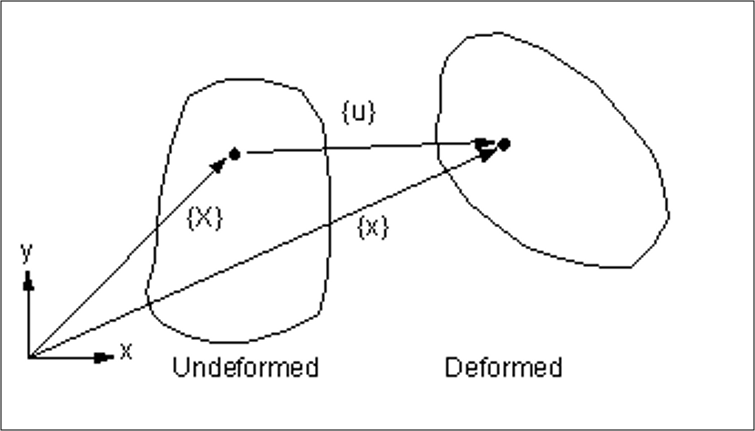
\includegraphics[height=3cm]{deformovane-nedeformovane-souradnice}
	\caption{Rozměry elementu}
\end{figure}

U~velkých deformací jsou však skutečné (deformované) rozměry podstatně odlišné od původních a~to je třeba respektovat.
Proto jsou zavedeny různé definice tenzorů přetvoření i~napětí.

\subsection{Tenzory popisující stav deformace v~bodě tělesa}
\begin{itemize}
	\item Pro malé deformace -- smluvní přetvoření (engineering strain)
	\item Green-Lagrangeův tenzor přetvoření
	\item Almansiho-Hamelův tenzor přetvoření
	\item Cauchyho (logaritmický) tenzor přetvoření
	\item Tenzor deformačního gradientu
	\item Cauchy-Greenův tenzor deformace (pravý a~levý)
	\item Tenzor protažení (stretch tensor)
\end{itemize}

Pro praktické použití jsou důležité vztahy pro vzájemný převod jednotlivých tenzorů přetvoření.

\subsection{Tenzory popisující napjatost v~bodě tělesa}
\begin{itemize}
	\item Piola-Kirchhoffův tenzor napětí 1.~druhu
	\item Cauchyho tenzor napětí (skutečná napětí -- true stress)
	\item Piola-Kirchhoffův tenzor napětí 2.~druhu
\end{itemize}

Pro správné (jednoznačné) určení energie napjatosti je nutné pracovat se vzájemně si odpovídajícími tenzory napětí a~přetvoření.
Těmto dvojicím tenzorů říkáme energeticky konjugované tenzory.
Takto konjugované jsou např.:
\begin{itemize}
	\item Green-Lagrangeův tenzor přetvoření a~2.~Piola-Kirchhoffův tenzor napětí,
	\item Pravý Cauchy-Greenův tenzor deformace a~2.~Piola-Kirchhoffův tenzor napětí,
	\item Pro praktické použití jsou důležité vztahy pro vzájemný převod jednotlivých tenzorů napětí.
\end{itemize}

\subsection{Vymezení hyperelastických materiálů}
Definice hyperelastického materiálu:
Materiál nazýváme hyperelastickým, pokud existuje elastická potenciální funkce $W$ (měrná deformační energie), která je skalární funkcí některého z~tenzorů přetvoření, resp. deformace a~jejíž parciální derivace podle některé složky přetvoření pak určuje odpovídající složku napětí.

To lze vyjádřit např. následovně:
\begin{equation}
	S_{ij} = \frac{\partial W}{\partial E_{ij}} = 2 \frac{\partial W}{\partial C_{ij}},
\end{equation}
kde
\begin{description}
	\item[$S_{ij}$] jsou složky 2.~Piola-Kirchhoffova tenzoru napětí
	\item[$W$] je funkce měrné energie napjatosti na jednotku nedeformovaného objemu
	\item[$E_{ij}$] jsou složky Green-Lagrangeova tenzoru přetvoření
	\item[$C_{ij}$] jsou složky pravého Cauchy-Greenova deformačního tenzoru
\end{description}

Kontrolní otázka: Vyhovuje této definici hyperelasticity hookovský materiál? Odpověď.
%todo zde prezentace energie-otazka-ppt

\subsection{Výpočet Cauchyho napětí u~hyperelastických materiálů}
Přepočet mezi tenzory napětí lze vyjádřit následovně:
\begin{equation}\label{key}
\sigma_{ij} = \frac{\rho}{\rho_0} F_{iR} S_{RS} F_{jS},
\end{equation}
kde
\begin{description}
	\item[$S_{RS}$] jsou složky 2.~Piola-Kirchhoffova tenzoru napětí,
	\item[$\sigma_{ij}$] jsou složky Cauchyho tenzoru (skutečného) napětí.
\end{description}

Napětí vypočítané parciální derivací je 2.~Piola-Kirchhoffovo, vynásobením  složkou tenzoru deformačního gradientu dostaneme postupně 1.~Piola-Kirchhoffovo a~Cauchyho napětí (odpovídá přepočtu mezi tenzory napětí).
Tak dostaneme vztah platný pro nestlačitelný materiál.
Protože však je měrná energie napjatosti $W$ vztažena na jednotku objemu v~nedeformovaném stavu, pro stlačitelný materiál (objem se mění) je nutno výsledek vynásobit poměrem měrných hmotností, kde $\rho_0$ odpovídá nedeformovanému a~$\rho$ deformovanému stavu.

\subsection{Rozdělení deformace na objemovou a~tvarovou složku}
U~všech hyperelastických konstitutivních modelů je stejně jako u~většiny ostatních třeba odděleně modelovat objemovou a~tvarovou (deviátorovou) složku deformace.
Proto konstitutivní vztahy sestávají ze dvou částí:
\begin{itemize}
	\item Vliv změny objemu na energii napjatosti popisují nejčastěji třetím invariantem tenzoru gradientu deformace $J$ a~konstantou popisující objemovou změnu (objemový modul pružnosti nebo jiná konstanta z~něj odvozená). Kromě pěnových gum je změna objemu malá oproti změně tvaru a~většinou vystačíme s~jejím lineárním popisem.
	\item Vliv tvarové změny se popisuje nejčastěji pomocí modifikovaných invariantů některého z tenzorů přetvoření. Modifikace má za cíl právě oddělení tvarové změny (deviátorové složky tenzoru) od změny objemové (kulová složka tenzoru).
\end{itemize}

\subsection{Přehled konstitutivních modelů respektujících velká přetvoření}
\subsubsection{Modely (hyper)elastické}
Izotropní (téměř) nestlačitelné: 
\begin{itemize}
	\item \hyperref[sec:neo-hooke]{Neo-Hooke}
	\item \hyperref[sec:mooney-rivlin]{Mooney-Rivlin}
	\item Klosner-Segal
	\item \hyperref[sec:yeoh]{Yeoh}
	\item \hyperref[sec:polynomicky-model]{Polynomial}
	\item Varga
	\item \hyperref[sec:model-ogden]{Ogden}
	\item Van der Waals
	\item \hyperref[sec:arruda-boyce]{Arruda-Boyce}
	\item Gent
	\item Pucci-Saccomandi
	\item Extended Tube
	\item Demiray
\end{itemize}

Izotropní stlačitelné
\begin{itemize}
	\item \hyperref[sec:ogden-foam]{Ogden (foam)}
	\item \hyperref[sec:blatz-ko]{Blatz-Ko (foam)}
	\item Hill-Storakers (foam)
\end{itemize}

\hyperref[sec:anizotropni-hyperelasticke-modely]{Anizotropní (téměř) nestlačitelné}
\begin{itemize}
	\item \hyperref[sec:polynomicky-anizotropni-hyperelasticky-model]{Polynomický}
	\item Fung
	\item Choi-Vito
	\item \hyperref[sec:model-hgo]{Holzapfel, 2000}
	\item Holzapfel, 2005
	\item Gasser (rozptyl směrů vláken, zjednodušená integrace)
	\item Microfiber (rozptyl směrů vláken, plná integrace)
\end{itemize}

\subsubsection{Modely neelastického chování}
Modely s~Mullinsovým efektem
\begin{itemize}
	\item \hyperref[sec:ogden-roxburgh]{Ogden-Roxburgh}
	\item Kachanov
	\item Miehe
	\item Marckmann
\end{itemize}

Visko-hyperelastické modely
\begin{itemize}
	\item \hyperref[sec:bergstrom-boyce]{Bergström-Boyce}
\end{itemize}

Elasto-plastické modely
\begin{itemize}
	\item \hyperref[sec:ramberg-osgood]{Ramberg-Osgood}
	\item \hyperref[sec:chaboche]{Chaboche}
\end{itemize}

Creepové modely
\begin{itemize}
	\item \hyperref[sec:norton]{Norton}
\end{itemize}

\subsubsection{Model Neo-Hooke}
Tento model zavádí měrnou energii napjatosti ve tvaru\footnote{(Treloar, 1975, pro nestlačitelnost odvozen termodynamicky již 1934)}
\begin{equation}\label{neo_hooke}
	W = \frac{G}{2} \left( \bar{I}_1 - 3 \right) + \frac{1}{d} \left( J - 1 \right)^2,
\end{equation}
kde
\begin{description}
	\item[$G$] je počáteční modul pružnosti ve smyku, přičemž platí $G = 2nkT$, kde $n$ je počet molekulárních řetězců v~jednotkovém objemu, $k$~je Boltzmanova konstanta a~$T$ je absolutní teplota,
	\item[$\bar{I}_1$] je modifikovaný první invariant pravého Cauchy-Greenova tenzoru deformace,
	\item[$d$] je parametr stlačitelnosti materiálu, daný vztahem $d = \frac{2}{K}$, kde $K$ je objemový modul pružnosti,
	\item[$J$] je třetí invariant tenzoru deformačního gradientu.
\end{description}

Vzhledem k~tomu, že tvarová změna je u~tohoto modelu popsána jedinou elastickou konstantou, je tento model použitelný do cca \SI{30}{\percent}, kdy nelinearita není příliš výrazná. Model je lineární pro Cauchyho napětí a~levý Cauchy-Greenův deformační tenzor.

Platí $G = 2nkT$, kde $n$ je počet molekulárních řetězců v~jednotkovém objemu, $k$ je Boltzmanova konstanta a~$T$ absolutní teplota.

\subsubsection{Model Mooney-Rivlin 2-parametrický}
Tento model zavádí měrnou energii napjatosti ve tvaru
\begin{equation}
	W = c_{10} \left(\bar{I}_1 - 3\right) + c_{01} \left(\bar{I}_2 - 3\right) + \frac{1}{d} \left(J - 1\right)^2,
\end{equation}
kde
\begin{description}
	\item[$c10, c01$] jsou materiálové parametry,
	\item[$\bar{I}_1$] je modifikovaný první invariant pravého Cauchy-Greenova tenzoru deformace,
	\item[$\bar{I}_2$] je modifikovaný druhý invariant pravého Cauchy-Greenova tenzoru deformace,
	\item[$d$] je parametr stlačitelnosti materiálu, daný vztahem $d = \frac{2}{K}$, kde $K$ je objemový modul pružnosti,
	\item[$J$] je třetí invariant tenzoru deformačního gradientu.
\end{description}

Tento model je použitelný do cca \SI{100}{\percent} přetvoření, pokud křivka přetvoření-napětí nevykazuje inflexi.

\subsubsection{Model Mooney-Rivlin 5-parametrický}
Tento model zavádí měrnou energii napjatosti ve tvaru
\begin{equation}
	W
	= c_{10} \left(\bar{I}_1 - 3\right)
	+ c_{01} \left(\bar{I}_2 - 3\right)
	+ c_{20} \left(\bar{I}_1 - 3\right)^2
	+ c_{11} \left(\bar{I}_1 - 3\right) \left(\bar{I}_2 - 3\right)
	+ c_{02} \left(\bar{I}_2 - 3\right)^2
	+ \frac{1}{d} \left(J - 1\right)^2,
\end{equation}
kde
\begin{description}
	\item[$c10, c01, c_{20}, c_{11}, c_{02}$] jsou materiálové parametry,
	\item[$\bar{I}_1$] je modifikovaný první invariant pravého Cauchy-Greenova tenzoru deformace,
	\item[$\bar{I}_2$] je modifikovaný druhý invariant pravého Cauchy-Greenova tenzoru deformace,
	\item[$d$] je parametr stlačitelnosti materiálu, daný vztahem $d = \frac{2}{K}$, kde $K$ je objemový modul pružnosti,
	\item[$J$] je třetí invariant tenzoru deformačního gradientu.
\end{description}

Tento model je použitelný i~tehdy, když křivka přetvoření-napětí vykazuje inflexi.

\subsubsection{Model Mooney-Rivlin 9-parametrický}
Tento model zavádí měrnou energii napjatosti ve tvaru
\begin{multline}
W
= c_{10} \left(\bar{I}_1 - 3\right)
+ c_{01} \left(\bar{I}_2 - 3\right)
+ c_{20} \left(\bar{I}_1 - 3\right)^2
+ c_{11} \left(\bar{I}_1 - 3\right) \left(\bar{I}_2 - 3\right)
+ c_{02} \left(\bar{I}_2 - 3\right)^2\\
+ c_{30} \left(\bar{I}_1 - 3\right)^3
+ c_{21} \left(\bar{I}_1 - 3\right)^2 \left(\bar{I}_2 - 3\right)
+ c_{12} \left(\bar{I}_1 - 3\right) \left(\bar{I}_2 - 3\right)^2
+ c_{03} \left(\bar{I}_2 - 3\right)^3
+ \frac{1}{d} \left(J - 1\right)^2,
\end{multline}
kde
\begin{description}
	\item[$c10, c01, c_{20}, c_{11}, c_{02}, c_{30}, c_{21}, c_{12}, c_{03}$] jsou materiálové parametry,
	\item[$\bar{I}_1$] je modifikovaný první invariant pravého Cauchy-Greenova tenzoru deformace,
	\item[$\bar{I}_2$] je modifikovaný druhý invariant pravého Cauchy-Greenova tenzoru deformace,
	\item[$d$] je parametr stlačitelnosti materiálu, daný vztahem $d = \frac{2}{K}$, kde $K$ je objemový modul pružnosti,
	\item[$J$] je třetí invariant tenzoru deformačního gradientu.
\end{description}

Tento model je použitelný i~pro komplikované tvary křivek přetvoření-napětí.

\subsubsection{Model polynomický}\label{sec:polynomicky-model}
Tento model je zobecněním modelů Mooney-Rivlin.
Zavádí energii napjatosti ve tvaru
\begin{equation}
W
= \sum\limits_{i+j=1}^N c_{ij} \left(\bar{I}_1 - 3\right)^i \left(\bar{I}_2 - 3\right)^j
+ \sum\limits_{k=1}^M \frac{1}{d_k} \left(J - 1\right)^{2k},
\end{equation}
kde
\begin{description}
	\item[$c_{ij}$, $d_k$] jsou materiálové parametry,
	\item[$\bar{I}_1$] je modifikovaný první invariant pravého Cauchy-Greenova tenzoru deformace,
	\item[$\bar{I}_2$] je modifikovaný druhý invariant pravého Cauchy-Greenova tenzoru deformace,
	\item[$J$] je třetí invariant tenzoru deformačního gradientu.
\end{description}

Pro $M=1$ a $N= 1,2,3$ dostaneme jednotlivé modely Mooney-Rivlin.
U~těchto modelů je počáteční modul pružnosti ve smyku
\begin{equation}
	G = 2 \left(c_{10} + c_{01}\right).
\end{equation}
Pro počáteční objemový modul pružnosti zde platí vztah
\begin{equation}
	K = \frac{2}{d_1}.
\end{equation}

\subsubsection{Model Ogden}\label{sec:model-ogden}
Tento model zavádí energii napjatosti ve tvaru
\begin{equation}
	W
	= \sum\limits_{p=1}^N \frac{\mu_p}{\alpha_p} \left( \bar{\lambda}_1^{\alpha_p} + \bar{\lambda}_2^{\alpha_p} + \bar{\lambda}_3^{\alpha_p} - 3\right)
	+ \sum\limits_{p=1}^N \frac{1}{d_p} \left(J - 1\right)^{2p},
\end{equation}
kde
\begin{description}
	\item[$\mu_p, \alpha_p, d_p$] jsou materiálové parametry,
	\item[$\bar{\lambda}_i (i=1,2,3)$] jsou modifikovaná hlavní poměrná protažení, složky levého Cauchy-Greenova tenzoru deformace,
	\item[$J$] je třetí invariant tenzoru deformačního gradientu.
\end{description}

Pro $N = 1$ a~$\alpha_p = 2$ dostaneme model Neo-Hooke.

U~obecného Ogdenova modelu je počáteční modul pružnosti ve smyku
\begin{equation}
	G = \frac{1}{2} \sum\limits_{p=1}^1 \alpha_p \cdot \mu_p.
\end{equation}
Pro počáteční objemový modul pružnosti zde platí vztah
\begin{equation}
	K = \frac{2}{d_1}.
\end{equation}

Tento model dokáže popsat i~extrémně velké deformace.

\subsection{Zadávání vlastností hyperelastických materiálů v~programových systémech MKP}
Existují dvě základní možnosti zadávání vlastností hyperelastického materiálu do programových systémů MKP:
\begin{itemize}
	\item Pomocí zadání experimentálních závislostí napětí-přetvoření, z~nichž program vypočítá materiálové parametry zvoleného modelu. Volbu vhodného modelu provádíme obvykle na základě vizuálního porovnání experimentálních a~vypočtených křivek a~na základě vyčíslení celkové energetické chyby modelu.
	\item Pomocí přímého zadání elastických parametrů zvoleného modelu. Tento způsob lze použít:
	\begin{itemize}
		\item Při opakovaných výpočtech s materiálem, jehož konstanty jsme již dříve určili; vhodné jen při nepříliš odlišných deformačně-napěťových stavech.
		\item Pokud jsme konstanty modelu určili z~experimentů jiným způsobem. Základem výpočtu konstant je metoda nejmenších čtverců, která hledá hodnoty konstant při minimalizaci kvadrátů odchylek. Při samostatném určování materiálových parametrů je možné použít sofistikovanější metody jejich určování, např. relativní odchylky místo absolutních, zvýraznění nebo potlačení některých částí deformačně napěťových křivek pomocí váhových koeficientů nebo změnou počtu zadávaných bodů experimentálních křivek (viz \texttt{www.hyperfit.wz.cz}).
	\end{itemize}
\end{itemize}

\subsection{Vstupní údaje potřebné pro identifikaci konstant hyperelastických modelů}
Pro určení materiálových parametrů se používají následující typy zkoušek:
\begin{enumerate}
	\item Zkouška jednoosým tahem (v~jednoosé tahové napjatosti)
	\item Zkouška jednoosým tlakem (v~jednoosé tlakové napjatosti)
	\item Zkouška ekvibiaxiální (ve dvouosé rovnoměrné napjatosti)
	\item Zkouška smykem nebo krutem (ve smykové napjatosti)
	\item Zkouška tahem při nulových příčných posuvech (v~rovinné deformaci)
	\item Zkouška tlakem při nulových příčných posuvech (v~rovinné deformaci)
	\item Zkouška objemové stlačitelnosti (v~trojosé rovnoměrné napjatosti)
\end{enumerate}
Některé z~těchto zkoušek je v~praxi velmi obtížné realizovat (např. zkouška prostým smykem -- při velkých deformacích vznikají i~normálová napětí, zkouška krutem na tenkostěnné trubce pro vyvolání homogenní smykové napjatosti zase vede ke ztrátě tvarové stability).
Některé ze zkoušek jsou však pro nestlačitelný materiál vzájemně rovnocenné. Proto se v praxi provádějí jen některé z~nich.

Proč jsou nutné zkoušky ve víceosé napjatosti?

\subsection{Základní zkoušky pro identifikaci konstant hyperelastických modelů}
Pro určení materiálových parametrů hyperelastických konstitutivních modelů se v praxi nejčastěji používají následující základní typy zkoušek:
\begin{itemize}
	\item Zkouška jednoosým tahem (v~jednoosé tahové napjatosti). Realizuje se na běžných zkušebních strojích pro tahovou zkoušku na plochých normalizovaných vzorcích ve tvaru oboustranné lopatky.
	\item Zkouška ekvibiaxiální (ve dvouosé rovnoměrné napjatosti). Realizuje se na speciálních zkušebních strojích na plochých vzorcích kruhového nebo čtvercového tvaru.
	\item Zkouška tahem při nulových příčných posuvech (v~rovinné deformaci). Realizuje se na běžných zkušebních strojích pro tahovou zkoušku s~použitím velmi širokých čelistí na plochých vzorcích obdélníkového tvaru s~velmi malým poměrem délky ku šířce (cca 0,1).
	\item Zkouška objemové stlačitelnosti (v~trojosé rovnoměrné napjatosti). Realizuje se na běžných zkušebních strojích pro zkoušku tahem a tlakem na válcových vzorcích  (nejčastěji průměr $29mm$, výška cca $13mm$), vtlačovaných těsným pístem do ocelové komůrky stejného tvaru a~rozměrů.
\end{itemize}

\subsection{Zadávání výsledků zkoušky do programových systémů MKP}
Většina současných komerčních programových systémů MKP disponuje softwarem pro identifikaci materiálových parametrů jednotlivých hyperelastických modelů z naměřených experimentálních křivek napětí-přetvoření. Při jejich zadávání je třeba mít na paměti následující upozornění:
\begin{itemize}
	\item Rozsah zkoušek (extrémní velikost přetvoření) by měl mírně přesahovat očekávaný rozsah přetvoření v~řešeném výpočtovém modelu. Obvykle jej předem neznáme, jedná se tedy o~iterační proces, kdy v~prvním kroku zadáme raději maximální změřený rozsah přetvoření a~na základě výsledků jej poté upravujeme. Příliš velký rozsah modelu totiž významně snižuje jeho přesnost.
	\item Nemáme-li k~dispozici výsledky všech potřebných materiálových zkoušek, je velmi riskantní používání zdánlivě přesnějších modelů používajících např. polynomy vyšších stupňů. Dosáhneme tím sice přesnější aproximace zadaných křivek, ale výsledky pro jiné typy napjatosti mohou být zcela nesmyslné (nejsou podloženy experimentálními daty). Zásadně je možné takový výpočtový model použít jen pro řešení takových problémů, při nichž se nevyskytnou typy deformačně-napěťových stavů, pro něž nebyly zadány experimentální křivky. V~opačném případě mohou být výsledky zcela chybné, podobně jako když rozsah přetvoření při určitém typu napjatosti (např. při jednoosém tahu) přesáhne rozsah realizovaný při experimentu.
\end{itemize}

\subsection{Zásady pro práci s~hyperelastickými modely v~programových systémech MKP}
\begin{itemize}
	\item Vždy zevrubně prostudujeme manuál programu, abychom zjistili použitý tvar funkce pro energii napjatosti a~význam jednotlivých materiálových parametrů, což je důležité pro jejich správné použití a~orientační kontrolu jejich hodnot.
	\item Zjistíme, v~jakých tenzorech napětí a~přetvoření je třeba zadávat experimentální údaje.
	\item Zjistíme, v~jakých tenzorech napětí a~přetvoření obdržíme konečné výsledky. 
	\item Při každé práci s~novým konstitutivním modelem nebo novým programovým systémem vždy nejprve provedeme simulaci základních zadaných zkoušek materiálu, abychom na úloze se známými výsledky eliminovali chybný postup při tvorbě a~zadávání modelu.
\end{itemize}
